\chapter{Results}
This chapter presents the empirical findings derived from the data collection process to address the research questions and expectations of the study. The research aims to evaluate the short-term impact of a school-based educational intervention designed to challenge traditional gender stereotypes in mathematics and introduce students to female mathematicians.

To provide a comprehensive evaluation, the results are organized into sequential analytical sections. First, the preparation of the dataset and descriptive statistics are reported, followed by reliability analyses of the instruments. Subsequently, baseline comparisons at $T_0$ and the main inferential analyses—including mixed ANOVAs and paired-sample t-tests—are presented to explore the effects of the intervention over time. Finally, exploratory analyses regarding the effect of age or grade, along with complementary qualitative data, are detailed to provide a complete interpretative context.

\section{Dataset preparation}
\subsection{Data Cleaning}
The initial sample consisted of 362 students from the selected middle school in Trieste. Prior to conducting inferential analyses, the dataset underwent a screening and cleaning process to ensure data integrity and the validity of the within-subjects design. The exclusion criteria were applied as follows:
\begin{enumerate}
    \item Missing Gender Information: Two participants did not disclose their gender These individuals were retained in the overall sample for descriptive statistics but were excluded from analyses requiring gender-based comparisons.
    \item Missing Pre–Post Correspondence: Questionnaires that could not be matched between the pre-test ($T_0$) and post-test ($T_1$) due to missing or invalid alphanumeric ID codes, or missing data from either session (e.g., due to student absence on the day of the intervention or follow-up), were removed from the dataset.
\end{enumerate}
The final matched dataset after these exclusions was utilized for the subsequent paired-sample comparisons and mixed ANOVA models.
\subsection{Coding and Scoring}
To prepare the composite variables for analysis, the dataset was processed according to the following psychometric procedures:
\begin{enumerate}
    \item Reverse Coding: Negatively worded items (such as "I would prefer not to have math lessons" in the Attitudes Toward Mathematics scale) were reverse-coded prior to computing the composite scores. This ensured that higher values consistently represented higher levels of the measured construct.
    \item Computation of Composite Variables: Composite scores for each construct were calculated by taking the mean of the responses across the items belonging to each scale. The composite variables were computed for both the pre-test and post-test conditions, resulting in the following measures with a theoretical range of 1 to 5:
    \begin{enumerate}
        \item $\text{Ansia\_Pre}$ and $\text{Ansia\_Post}$ (Math Anxiety)
        \item $\text{Autoefficacia\_Pre}$ and $\text{Autoefficacia\_Post}$ (Mathematics Self-Efficacy)
        \item $\text{Atteggiamenti\_Pre}$ and $\text{Atteggiamenti\_Post}$ (Attitudes Toward Mathematics)
        \item $\text{Stereotipi\_Pre}$ and $\text{Stereotipi\_Post}$ (Gender Stereotypes in Mathematics)
    \end{enumerate}
\end{enumerate}
\section{Sample Description}
The sample for the study comprises $N = 362$ students from a middle school (scuola secondaria di primo grado) located in the city center of Trieste, which serves a total population of approximately 533 students. The participants and the participating classes were selected using purposive sampling based on teacher willingness and scheduling compatibility.The sample is distributed across the three grade levels of the school: 127 students from Grade 6, 121 students from Grade 7, and 114 students from Grade 8. The descriptive statistics of the participants, categorized by gender, are summarized in the table below.
\begin{table}[htbp]
  \centering
  \caption{Summary of age by gender and school year (Section 5.2)}
  \label{tab:age_gender_long}
  \begin{tabular}{lcc}
    \toprule
    Gender & School Year & N \\
    \midrule
    F & 1 & 62 \\
      & 2 & 62 \\
      & 3 & 50 \\
    \addlinespace
    M & 1 & 63 \\
      & 2 & 59 \\
      & 3 & 64 \\
    \addlinespace
    O & 1 & 2 \\
      & 2 & 0 \\
      & 3 & 0 \\
    \bottomrule
  \end{tabular}
\end{table}
\section{Reliability Analysis}
To verify the internal consistency of the instruments used in the study, Cronbach's alpha coefficients ($\alpha$) were calculated for the four scales at the pre-test stage ($T_1$). Following standard methodological guidelines, a reliability coefficient of $\alpha \ge .70$ was considered good, while values of $\alpha \ge .60$ were considered acceptable for an exploratory study.The internal consistency values for the four composite constructs are presented in the table below.
\begin{table}[htbp]
  \centering
  \caption{Reliability of the Scales at Baseline ($T_1$)}
  \label{tab:reliability_baseline}
  \begin{tabular}{lcc}
    \toprule
    Scale & Number of Items & Cronbach's alpha ($\alpha$) \\
    \midrule
    Math Anxiety & 9 & 0.826 \\
    Mathematics Self-Efficacy & 10 & 0.820 \\
    Attitudes Toward Mathematics & 8 & 0.852 \\
    Gender Stereotypes in Mathematics & 9 & 0.815 \\
    \bottomrule
  \end{tabular}
\end{table}
All scales demonstrated good internal consistency, well above the acceptable threshold, permitting further inferential analysis.
\section{Preliminary Analysis (Baseline $T_1$)}
\subsection{Gender Comparisons at Baseline}
To determine whether there were any significant differences between male and female students prior to the educational intervention, independent samples t-tests were conducted on the four composite baseline measures: Math Anxiety, Mathematics Self-Efficacy, Attitudes Toward Mathematics, and Gender Stereotypes.

As noted in the dataset preparation, the two students who did not disclose their gender were excluded from this baseline analysis. Both Student's t-test and Welch's t-test (to account for unequal variances) were performed. The alternative hypothesis tested was $H_a: \mu_F \neq \mu_M$.
The descriptive statistics for each group are summarized in Table~\ref{tab:descriptives_baseline}.

\begin{table}[htbp]
\centering
\caption{Group Descriptives for Baseline Measures by Gender}
\label{tab:descriptives_baseline}
\begin{tabular}{lccccc}
\hline
Construct & Group & N & Mean & SD & SE \\
\hline
Math Anxiety & F & 165 & 2.74 & 0.70 & 0.05 \\
& M & 176 & 2.37 & 0.70 & 0.05 \\
\hline
Mathematics Self-Efficacy & F & 171 & 3.39 & 0.66 & 0.05 \\
& M & 180 & 3.55 & 0.71 & 0.05 \\
\hline
Attitudes Toward Mathematics & F & 169 & 3.20 & 0.90 & 0.07 \\
& M & 180 & 3.48 & 0.79 & 0.06 \\
\hline
Gender Stereotypes & F & 169 & 1.35 & 0.54 & 0.04 \\
& M & 184 & 1.34 & 0.52 & 0.04 \\
\hline
\end{tabular}
\end{table}
The results of the independent samples t-tests are presented in the table below.

\begin{table}[htbp]
\centering
\caption{Independent Samples T-Test by Gender at Baseline}
\label{tab:ttest_baseline}
\begin{tabular}{lccccc}
\hline
Construct & Test Type & Statistic & df & p-value & Cohen's d \\
\hline
Math Anxiety & Student's t & 4.91 & 339 & < .001 & 0.53 \\
& Welch's t & 4.91 & 338 & < .001 & 0.53 \\
\hline
Mathematics Self-Efficacy & Student's t & -2.25 & 349 & .025 & -0.24 \\
& Welch's t & -2.26 & 349 & .025 & -0.24 \\
\hline
Attitudes Toward Mathematics & Student's t & -3.12\textsuperscript{a} & 347 & .002 & -0.33 \\
& Welch's t & -3.11 & 335 & .002 & -0.33 \\
\hline
Gender Stereotypes & Student's t & 0.08 & 351 & .935 & 0.01 \\
& Welch's t & 0.08 & 345 & .935 & 0.01 \\
\hline
\end{tabular}
\end{table}

\textsuperscript{a} \textit{Note: Levene's test is significant ($p < .05$), suggesting a violation of the assumption of equal variances.}

Regarding the baseline comparisons between genders, the analysis of Math Anxiety revealed a statistically significant difference between male and female students, with $t(339) = 4.91, p < .001$, reflecting a medium effect size ($d = 0.53$). Specifically, female students reported higher levels of anxiety ($M = 2.74, SD = 0.70$) compared to male students ($M = 2.37, SD = 0.70$). A statistically significant difference was also found in Mathematics Self-Efficacy, $t(349) = -2.25, p = .025$, indicating a small effect size ($d = -0.24$), with females scoring $M = 3.39, SD = 0.66$ and males scoring $M = 3.55, SD = 0.71$. Similarly, the analysis of the Attitudes Toward Mathematics scale indicated a significant difference between genders, $t(347) = -3.12, p = .002$, with a small effect size ($d = -0.33$). Due to a violation of the assumption of equal variances for this construct, a Welch's t-test was also considered, which confirmed the result ($t = -3.11, df = 335, p = .002$). Here, female students showed a lower attitude score ($M = 3.20, SD = 0.90$) compared to male students ($M = 3.48, SD = 0.79$). Conversely, there was no statistically significant difference between genders regarding the Gender Stereotypes construct, $t(351) = 0.08, p = .935$, where the effect size was found to be negligible ($d = 0.01$, females: $M = 1.35, SD = 0.54$; males: $M = 1.34, SD = 0.52$).
\subsection{Correlations Between Constructs}

To evaluate the theoretical coherence among the measured constructs at baseline, Pearson correlation coefficients ($r$) were calculated across the four composite baseline variables. This analysis verifies the relationships established in the theoretical framework, particularly the inverse relationship between math anxiety and mathematics self-efficacy.

The correlation matrix for the baseline variables is presented in the table below.

\begin{table}[htbp]
\centering
\caption{Pearson Correlation Matrix at Baseline ($T_0$)}
\label{tab:corr_baseline}
\begin{tabular}{lcccc}
\hline
Construct & Math Anxiety & Self-Efficacy & Attitudes & Gender Stereotypes \\
\hline
Math Anxiety & 1.00 & & & \\
Mathematics Self-Efficacy & -0.444\textsuperscript{**} & 1.00 & & \\
Attitudes Toward Mathematics & -0.424\textsuperscript{**} & 0.603\textsuperscript{**} & 1.00 &  \\
Gender Stereotypes & 0.365\textsuperscript{**} & -0.185\textsuperscript{**} & -0.171\textsuperscript{**} & 1.00 \\
\hline
\end{tabular}
\end{table}

\textsuperscript{*} \textit{Correlation is significant at the $p < 0.05$ level.} \\
\textsuperscript{**} \textit{Correlation is significant at the $p < 0.001$ level.}

\subsubsection*{Findings}
The analysis of the baseline correlations indicated a significant negative relationship between math anxiety and mathematics self-efficacy ($r = -0.444, p < .001$). Furthermore, a significant negative correlation was found between math anxiety and attitudes toward mathematics ($r = -0.424, p < .001$). A strong positive correlation emerged between self-efficacy and attitudes toward mathematics ($r = 0.603, p < .001$). Regarding gender stereotypes, a significant positive correlation was observed with math anxiety ($r = 0.365, p < .001$), whereas significant negative correlations were found with both self-efficacy ($r = -0.185, p < .001$) and attitudes toward mathematics ($r = -0.171, p = .001$).

\section{Main Findings: Effects of the Intervention}

To evaluate the short-term impact of the educational intervention, mixed-design Analysis of Variance (ANOVA) models were conducted for each of the four primary constructs: Math Anxiety, Mathematics Self-Efficacy, Attitudes Toward Mathematics, and Gender Stereotypes. Each model evaluated the within-subject factor of Time (Pre-test vs. Post-test) and the between-subject factor of Gender (Female vs. Male). As noted in the dataset preparation, the two participants who did not disclose their gender were excluded from the between-subject analyses. Before applying the ANOVAs, the assumption of normality was assumed to hold approximately due to the sample size, in accordance with the Central Limit Theorem, and Levene's test was examined to evaluate the homogeneity of variances. The results of the mixed ANOVAs are summarized in Table~\ref{tab:anova_results}.

\begin{table}[htbp]
\centering
\small
\caption{Mixed ANOVA Results for the Measured Constructs}
\label{tab:anova_results}
\begin{tabularx}{\textwidth}{l|l|cccr}
\hline
\textbf{Construct} & \textbf{Effect} & \textbf{df} & \textbf{F} & \textbf{p} & \textbf{\boldmath$\eta^2_p$} \\
\hline
\multirow{3}{*}{Math Anxiety} 
& Time & 1, 330 & 12.55 & < .001 & 0.037 \\
& Time $\times$ Gender & 1, 330 & 0.59 & .445 & 0.002 \\
& Gender & 1, 330 & 23.20 & < .001 & 0.066 \\
\hline
\multirow{3}{*}{Math Self-Efficacy} 
& Time & 1, 340 & 3.11 & .079 & 0.009 \\
& Time $\times$ Gender & 1, 340 & 0.50 & .482 & 0.001 \\
& Gender & 1, 340 & 6.95 & .009 & 0.020 \\
\hline
\multirow{3}{*}{Attitudes Toward Math} 
& Time & 1, 339 & 4.24 & .040 & 0.012 \\
& Time $\times$ Gender & 1, 339 & 1.08 & .300 & 0.003 \\
& Gender & 1, 339 & 7.80 & .006 & 0.022 \\
\hline
\multirow{3}{*}{Gender Stereotypes} 
& Time & 1, 349 & 33.63 & < .001 & 0.088 \\
& Time $\times$ Gender & 1, 349 & 0.14 & .713 & 0.000 \\
& Gender & 1, 349 & 0.03 & .863 & 0.000 \\
\hline
\end{tabularx}
\end{table}

\subsubsection*{Math Anxiety}
Regarding math anxiety, the mixed ANOVA yielded a statistically significant main effect of time, $F(1, 330) = 12.55, p < .001, \eta^2_p = 0.037$, showing that anxiety levels changed significantly following the educational intervention. The interaction effect between time and gender was not statistically significant, $F(1, 330) = 0.59, p = .445, \eta^2_p = 0.002$, which indicates that the intervention's effect on anxiety did not differ significantly between male and female students. Furthermore, a significant main effect of gender was observed, $F(1, 330) = 23.20, p < .001, \eta^2_p = 0.066$. Levene's test for equality of variances was not significant for either time point, confirming the assumption of homogeneity of variance. 

\begin{figure}[H]
\centering
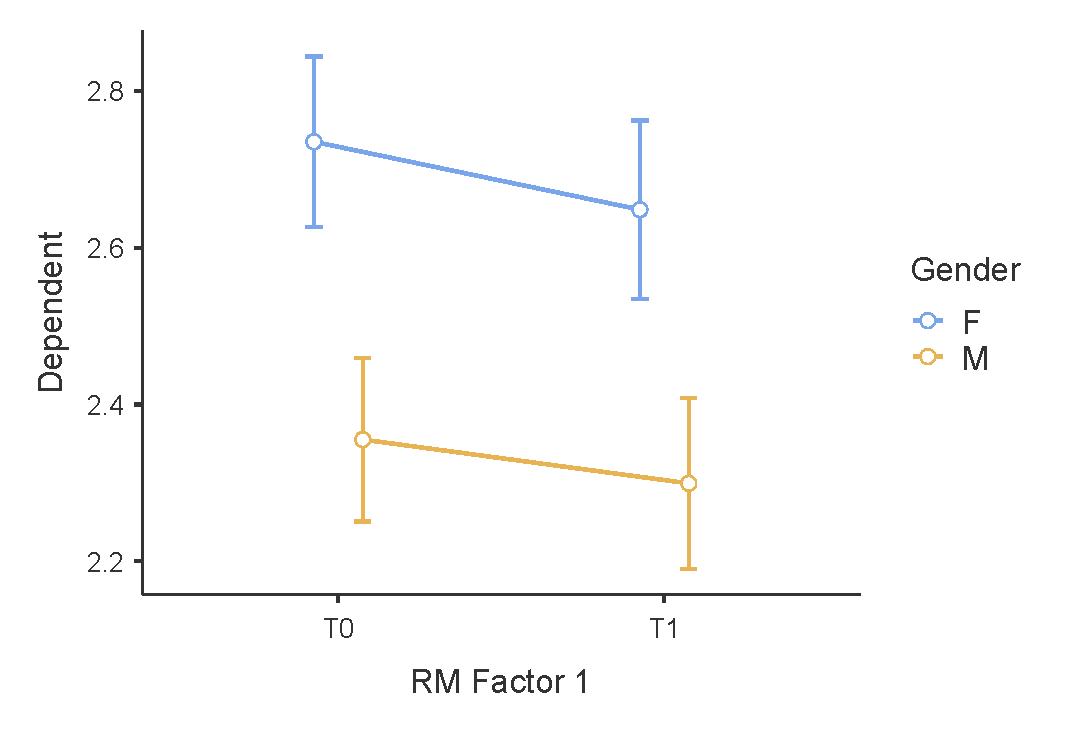
\includegraphics[width=0.75\textwidth]{img/Ch5/Estimated Marginal Means Anxiety.pdf}
\caption{Marginal means over time for Math Anxiety by Gender.}
\label{fig:ansia}
\end{figure}

\subsubsection*{Mathematics Self-Efficacy}
The analysis for mathematics self-efficacy indicated that the main effect of time did not reach conventional levels of statistical significance, $F(1, 340) = 3.11, p = .079, \eta^2_p = 0.009$. Similarly, the interaction effect between time and gender was not statistically significant, $F(1, 340) = 0.50, p = .482, \eta^2_p = 0.001$. However, the analysis revealed a significant main effect of gender, $F(1, 340) = 6.95, p = .009, \eta^2_p = 0.020$. Assumptions regarding the homogeneity of variances were met, as confirmed by Levene's test. 

\begin{figure}[H]
\centering
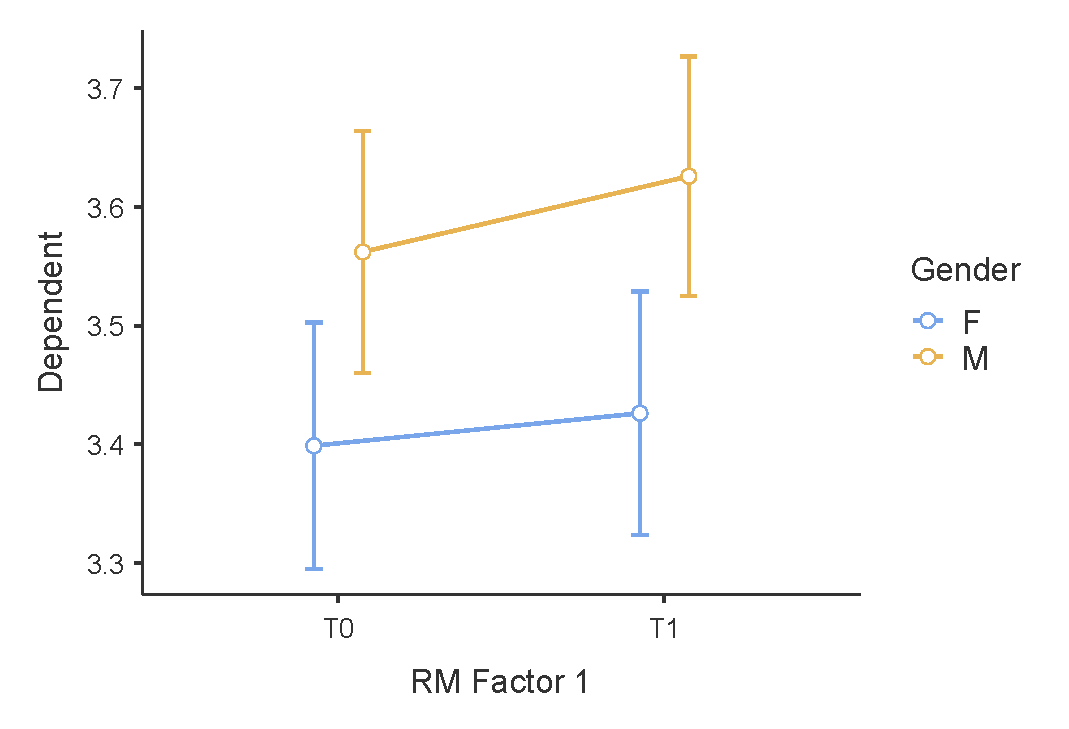
\includegraphics[width=0.75\textwidth]{img/Ch5/Estimated Marginal Means Self-Efficacy.pdf} 
\caption{Marginal means over time for Mathematics Self-Efficacy by Gender.}
\label{fig:autoefficacia}
\end{figure}

\subsubsection*{Attitudes Toward Mathematics}
For attitudes toward mathematics, the mixed ANOVA showed a significant main effect of time, $F(1, 339) = 4.24, p = .040, \eta^2_p = 0.012$, signifying a meaningful change over time. The interaction between time and gender was not statistically significant, $F(1, 339) = 1.08, p = .300, \eta^2_p = 0.003$. In addition, the main effect of gender was found to be significant, $F(1, 339) = 7.80, p = .006, \eta^2_p = 0.022$. Levene's test was significant at the pre-test measurement ($p = .046$), suggesting a slight violation of the assumption of equal variances, though the model is generally robust to this deviation. 

\begin{figure}[H]
\centering
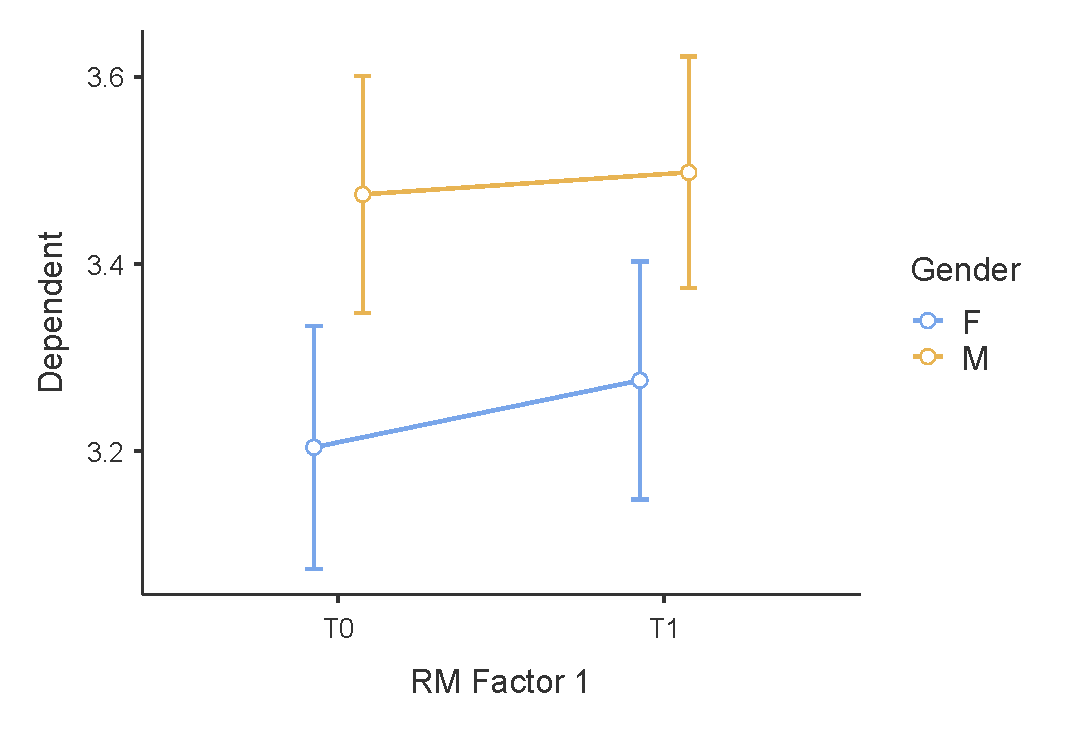
\includegraphics[width=0.75\textwidth]{img/Ch5/Estimated Marginal Means Attitudes.pdf}
\caption{Marginal means over time for Attitudes Toward Mathematics by Gender.}
\label{fig:atteggiamenti}
\end{figure}

\subsubsection*{Gender Stereotypes}
The analysis of the gender stereotypes construct revealed a statistically significant main effect of time, $F(1, 349) = 33.63, p < .001, \eta^2_p = 0.088$, demonstrating a substantial change after the educational seminar. The interaction effect between time and gender was not statistically significant, $F(1, 349) = 0.14, p = .713, \eta^2_p = 0.000$. The main effect of gender was also not significant, $F(1, 349) = 0.03, p = .863, \eta^2_p = 0.000$. Levene's test was not significant at either time point, ensuring the homogeneity of variances. 

\begin{figure}[H]
\centering
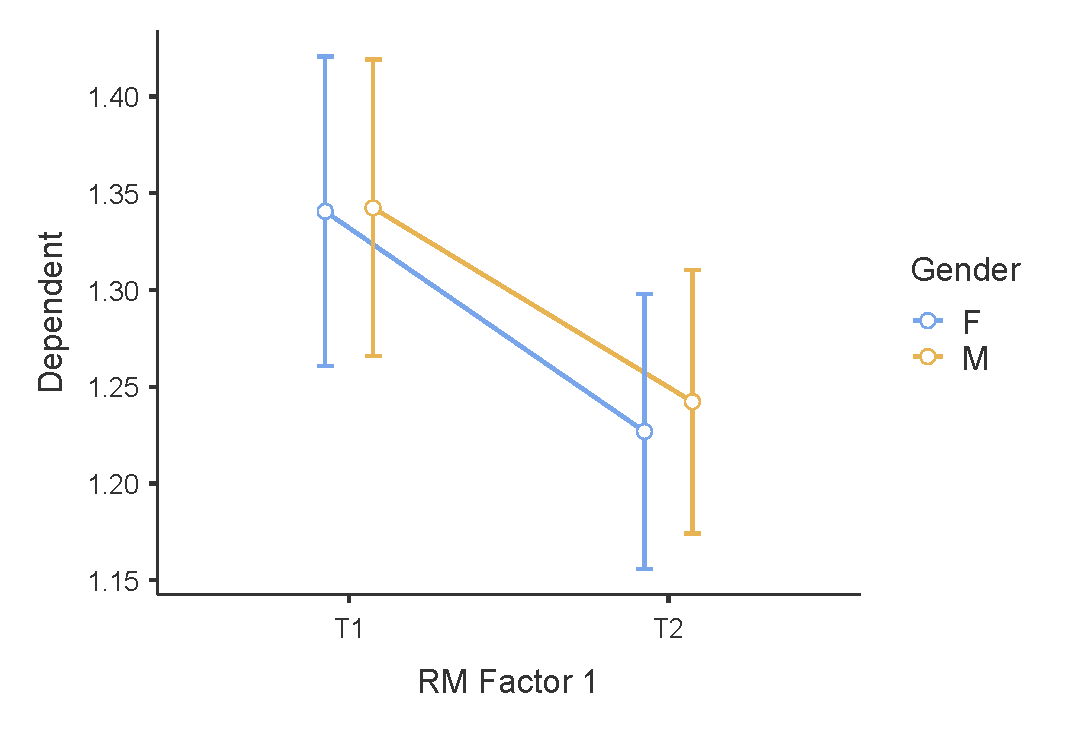
\includegraphics[width=0.75\textwidth]{img/Ch5/Estimated Marginal Means Stereotypes.pdf}
\caption{Marginal means over time for Gender Stereotypes by Gender.}
\label{fig:stereotipi}
\end{figure}

\subsection{Supplementary Analyses: Robustness Checks}

To ensure the robustness of the findings and to complement the mixed-design ANOVA models, paired-samples t-tests were conducted on the entire sample to compare the pre-test and post-test scores for each of the four primary constructs. Cohen's $d$ was computed as a measure of effect size for each comparison, and it is reported regardless of statistical significance to provide a complete picture of the intervention's impact. The results of the paired-samples t-tests and the corresponding effect sizes are summarized in Table~\ref{tab:ttest_results}.

\begin{table}[htbp]
\centering
\small
\caption{Paired-Samples T-Test Results and Effect Sizes}
\label{tab:ttest_results}
\begin{tabularx}{\textwidth}{l|ccccc}
\hline
\textbf{Construct} & \textbf{df} & \textbf{t} & \textbf{p} & \textbf{Mean Difference} & \textbf{Cohen's \boldmath$d$} \\
\hline
Math Anxiety & 331 & 3.52 & < .001 & 0.14 & 0.19 \\
Mathematics Self-Efficacy & 341 & -1.78 & .076 & -0.05 & -0.10 \\
Attitudes Toward Mathematics & 340 & -2.03 & .043 & -0.07 & -0.11 \\
Gender Stereotypes & 351 & 5.99 & < .001 & 0.23 & 0.32 \\
\hline
\end{tabularx}
\end{table}

\subsubsection*{Math Anxiety}
For math anxiety, the paired-samples t-test revealed a statistically significant difference between the pre-test and post-test scores, $t(331) = 3.52$, $p < .001$, with a small effect size (Cohen's $d = 0.193$). This confirms that the observed decrease in anxiety levels remains robust when examined across the entire sample.

\subsubsection*{Mathematics Self-Efficacy}
Consistent with the mixed ANOVA results, the paired-samples t-test for mathematics self-efficacy did not yield a statistically significant difference between the two time points, $t(341) = -1.78$, $p = .076$. The effect size was small (Cohen's $d = -0.096$), indicating only a marginal shift in self-efficacy for the overall sample.

\subsubsection*{Attitudes Toward Mathematics}
The t-test for attitudes toward mathematics showed a statistically significant difference between pre-test and post-test scores, $t(340) = -2.03$, $p = .043$. The effect size was small (Cohen's $d = -0.110$), confirming a slight negative shift over time for the overall sample.

\subsubsection*{Gender Stereotypes}
Finally, the paired-samples t-test for gender stereotypes demonstrated a statistically significant difference between the pre-test and post-test scores, $t(351) = 5.99$, $p < .001$, with a small-to-medium effect size (Cohen's $d = 0.319$). This indicates a robust and meaningful reduction in gender stereotypes following the educational intervention.



\subsection{Exploratory Analysis: Effect of Grade Level}

To explore whether the short-term impact of the educational intervention varied across different grade levels, one-way analysis of variance (ANOVA) tests were conducted. The independent variable was the grade level (Classes 1, 2, and 3), and the dependent variables were the difference scores calculated by subtracting the pre-test scores from the post-test scores ($T_1 - T_0$) for each of the four constructs: Math Anxiety, Mathematics Self-Efficacy, Attitudes Toward Mathematics, and Gender Stereotypes.

The results of the one-way ANOVA are summarized in Table~\ref{tab:anova_grade}.

\begin{table}[htbp]
\centering
\small
\caption{One-Way ANOVA of Difference Scores by Grade Level}
\label{tab:anova_grade}
\begin{tabularx}{\textwidth}{l|ccccc}
\hline
\textbf{Construct} & \textbf{df1} & \textbf{df2} & \textbf{F} & \textbf{p} \\
\hline
Math Anxiety Difference & 2 & 217 & 0.689 & .503 \\
Self-Efficacy Difference & 2 & 217 & 0.405 & .668 \\
Attitudes Difference & 2 & 223 & 0.344 & .709 \\
Gender Stereotypes Difference & 2 & 232 & 0.814 & .444 \\
\hline
\end{tabularx}
\end{table}

\subsubsection*{Math Anxiety}
The one-way ANOVA on the difference scores for math anxiety revealed no statistically significant differences across the grade levels, $F(2, 217) = 0.689, p = .503$. Post-hoc comparisons using the Tukey HSD test confirmed that there were no significant differences between Classes 1 and 2 ($p = .465$), Classes 1 and 3 ($p = .916$), or Classes 2 and 3 ($p = .728$). This suggests that the intervention's effect on math anxiety was consistent regardless of the students' grade level. Levene's test of equality of variances was significant, $F(2, 329) = 3.13, p = .045$, suggesting a violation of the assumption of equal variances, though the result remains robust. Figure~\ref{fig:ansia_diff} illustrates the mean difference scores and 95\% confidence intervals across the different school years.

\begin{figure}[htbp]
\centering
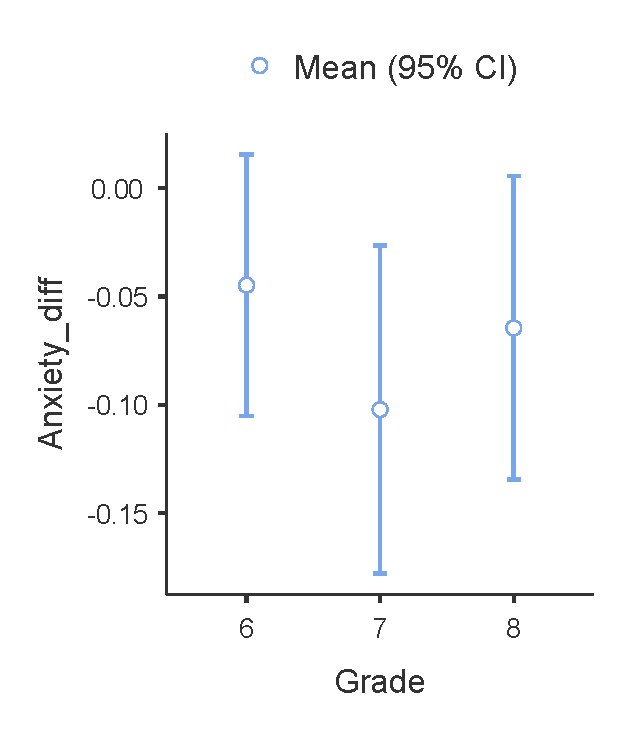
\includegraphics[width=0.75\textwidth]{img/Ch5/oneway anova anxiety.pdf}
\caption{Mean difference scores and 95\% confidence intervals for Math Anxiety by School Year.}
\label{fig:ansia_diff}
\end{figure}

\subsubsection*{Mathematics Self-Efficacy}
The one-way ANOVA on the difference scores for mathematics self-efficacy showed no statistically significant differences across the grade levels, $F(2, 217) = 0.405, p = .668$. Tukey HSD post-hoc tests indicated no significant differences between Classes 1 and 2 ($p = .802$), Classes 1 and 3 ($p = .999$), or Classes 2 and 3 ($p = .789$). This indicates that the change in self-efficacy was consistent across the school years. Levene's test of equality of variances was not significant, $F(2, 339) = 2.54, p = .080$, confirming the homogeneity of variance. Figure~\ref{fig:self_diff} illustrates the mean difference scores and 95\% confidence intervals.

\begin{figure}[htbp]
\centering
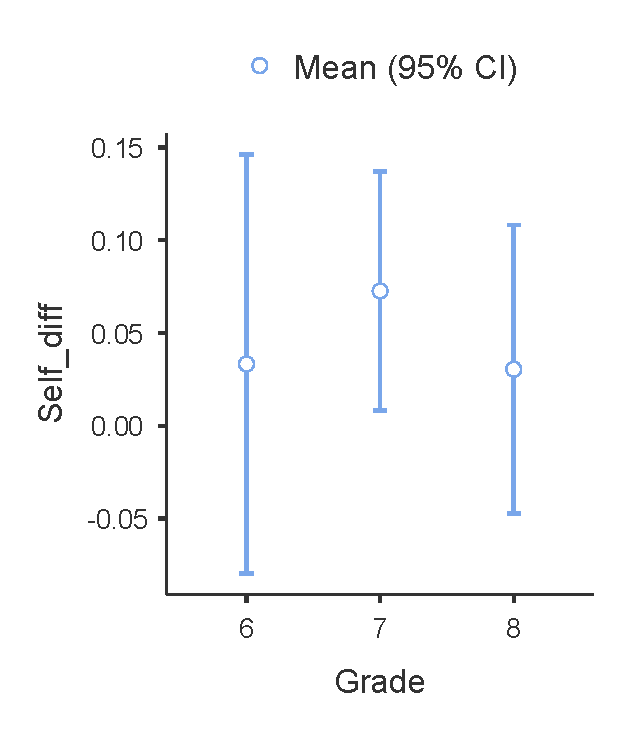
\includegraphics[width=0.75\textwidth]{img/Ch5/oneway anova selfefficacy.pdf}
\caption{Mean difference scores and 95\% confidence intervals for Mathematics Self-Efficacy by School Year.}
\label{fig:self_diff}
\end{figure}

\subsubsection*{Attitudes Toward Mathematics}
The one-way ANOVA on the difference scores for attitudes toward mathematics revealed no statistically significant differences across the grade levels, $F(2, 223) = 0.344, p = .709$. Post-hoc comparisons using the Tukey HSD test confirmed that there were no significant differences between Classes 1 and 2 ($p = .742$), Classes 1 and 3 ($p = .754$), or Classes 2 and 3 ($p = 1.000$). This suggests that the intervention's effect on attitudes was uniform across the grade levels. Levene's test of equality of variances was not significant, $F(2, 338) = 0.884, p = .414$, verifying the assumption of equal variances. Figure~\ref{fig:attitudes_diff} illustrates the mean difference scores across the school years.

\begin{figure}[htbp]
\centering
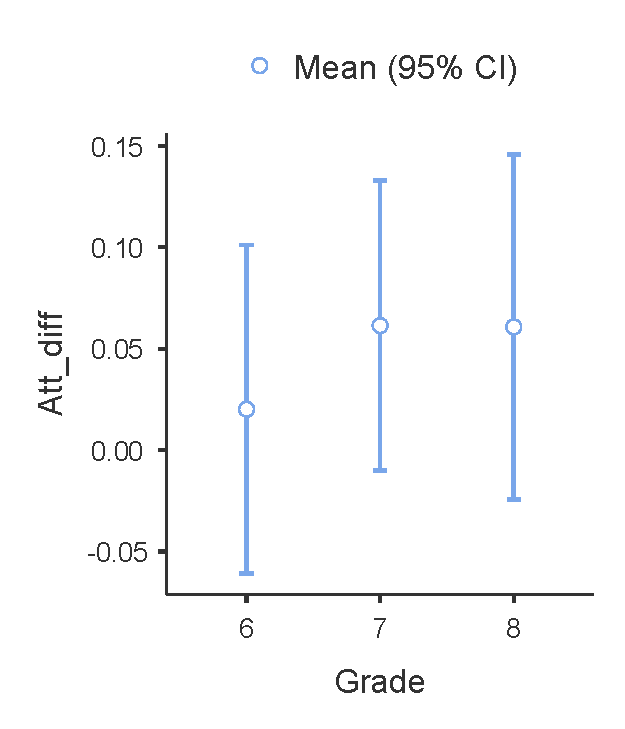
\includegraphics[width=0.75\textwidth]{img/Ch5/oneway anova attitudes.pdf}
\caption{Mean difference scores and 95\% confidence intervals for Attitudes Toward Mathematics by School Year.}
\label{fig:attitudes_diff}
\end{figure}

\subsubsection*{Gender Stereotypes}
The one-way ANOVA on the difference scores for gender stereotypes indicated no statistically significant differences across the grade levels, $F(2, 232) = 0.814, p = .444$. Tukey HSD post-hoc tests showed no significant differences between Classes 1 and 2 ($p = .399$), Classes 1 and 3 ($p = .734$), or Classes 2 and 3 ($p = .858$). This indicates that the intervention effect on gender stereotypes was consistent across the school years. Levene's test of equality of variances was not significant, $F(2, 348) = 0.471, p = .624$, confirming the homogeneity of variance. Figure~\ref{fig:stereotypes_diff} illustrates the mean difference scores across the school years.

\begin{figure}[htbp]
\centering
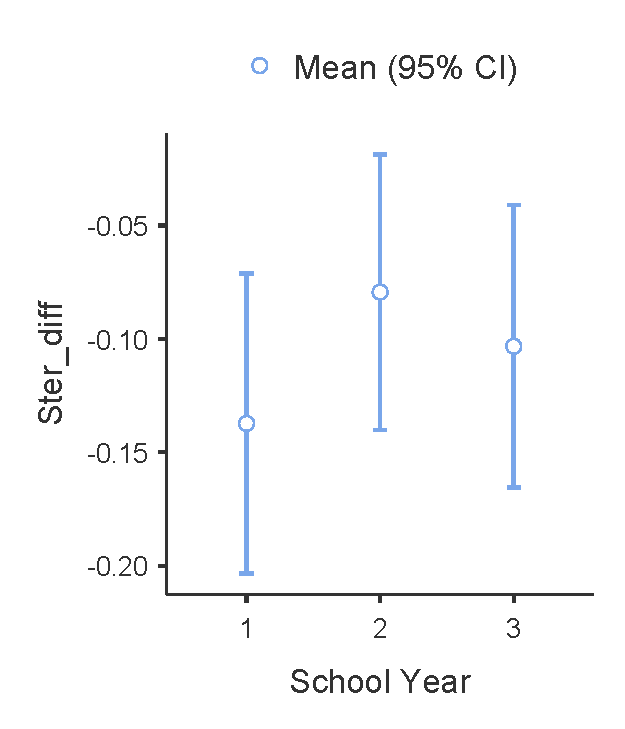
\includegraphics[width=0.75\textwidth]{img/Ch5/oneway anova stereotypes.pdf}
\caption{Mean difference scores and 95\% confidence intervals for Gender Stereotypes by School Year.}
\label{fig:stereotypes_diff}
\end{figure}